\documentclass[12pt]{article}

%packages
%\usepackage{latexsym}
\usepackage{graphicx}
\usepackage{wrapfig}
\usepackage{color}
\usepackage{amsmath}
%\usepackage{dsfont}
\usepackage{placeins}
\usepackage{amssymb}
\usepackage{skull}
\usepackage{enumerate}
\usepackage{soul}
\usepackage{alphalph}
\usepackage{hyperref}
%\usepackage{fancyhdr}

%\fancyhf{} % clear all header and footers
%\renewcommand{\headrulewidth}{0pt} % remove the header rule
%\fancyfoot[LE, LO]{\thepage}


%\usepackage{pstricks,pst-node,pst-tree}

%\usepackage{algpseudocode}
%\usepackage{amsthm}
%\usepackage{hyperref}
%\usepackage{mathrsfs}
%\usepackage{amsfonts}
%\usepackage{bbding}
%\usepackage{listings}
%\usepackage{appendix}
\usepackage[margin=1in]{geometry}
%\geometry{papersize={8.5in,11in},total={6.5in,9in}}
%\usepackage{cancel}
%\usepackage{algorithmic, algorithm}

\newcommand{\qu}[1]{``#1''}
\newcommand{\spc}[1]{\\ \vspace{#1cm}}

\newcounter{probnum}
\setcounter{probnum}{1}
\newcounter{numpts}
\setcounter{numpts}{0}

%create definition to allow local margin changes
\def\changemargin#1#2{\list{}{\rightmargin#2\leftmargin#1}\item[]}
\let\endchangemargin=\endlist 

%allow equations to span multiple pages
\allowdisplaybreaks

%define colors and color typesetting conveniences
\definecolor{gray}{rgb}{0.5,0.5,0.5}
\definecolor{black}{rgb}{0,0,0}
\definecolor{white}{rgb}{1,1,1}
\definecolor{blue}{rgb}{0.5,0.5,1}
\newcommand{\inblue}[1]{\color{blue}#1 \color{black}}
\definecolor{green}{rgb}{0.133,0.545,0.133}
\newcommand{\ingreen}[1]{\color{green}#1 \color{black}}
\definecolor{yellow}{rgb}{1,0.549,0}
\newcommand{\inyellow}[1]{\color{yellow}#1 \color{black}}
\definecolor{red}{rgb}{1,0.133,0.133}
\newcommand{\inred}[1]{\color{red}#1 \color{black}}
\definecolor{purple}{rgb}{0.58,0,0.827}
\newcommand{\inpurple}[1]{\color{purple}#1 \color{black}}
\definecolor{gray}{rgb}{0.5,0.5,0.5}
\newcommand{\ingray}[1]{\color{gray}#1 \color{black}}
\definecolor{backgcode}{rgb}{0.97,0.97,0.8}
\definecolor{Brown}{cmyk}{0,0.81,1,0.60}
\definecolor{OliveGreen}{cmyk}{0.64,0,0.95,0.40}
\definecolor{CadetBlue}{cmyk}{0.62,0.57,0.23,0}

%define new math operators
\DeclareMathOperator*{\argmax}{arg\,max~}
\DeclareMathOperator*{\argmin}{arg\,min~}
\DeclareMathOperator*{\argsup}{arg\,sup~}
\DeclareMathOperator*{\arginf}{arg\,inf~}
\DeclareMathOperator*{\convolution}{\text{\Huge{$\ast$}}}
\newcommand{\infconv}[2]{\convolution^\infty_{#1 = 1} #2}
%true functions

%%%% GENERAL SHORTCUTS

\makeatletter
\newalphalph{\alphmult}[mult]{\@alph}{26}
\renewcommand{\labelenumi}{(\alphmult{\value{enumi}})}
\renewcommand{\theenumi}{\AlphAlph{\value{enumi}}}
\makeatother
%shortcuts for pure typesetting conveniences
\newcommand{\bv}[1]{\boldsymbol{#1}}

%shortcuts for compound constants
\newcommand{\BetaDistrConst}{\dfrac{\Gamma(\alpha + \beta)}{\Gamma(\alpha)\Gamma(\beta)}}
\newcommand{\NormDistrConst}{\dfrac{1}{\sqrt{2\pi\sigma^2}}}

%shortcuts for conventional symbols
\newcommand{\tsq}{\tau^2}
\newcommand{\tsqh}{\hat{\tau}^2}
\newcommand{\sigsq}{\sigma^2}
\newcommand{\sigsqsq}{\parens{\sigma^2}^2}
\newcommand{\sigsqovern}{\dfrac{\sigsq}{n}}
\newcommand{\tausq}{\tau^2}
\newcommand{\tausqalpha}{\tau^2_\alpha}
\newcommand{\tausqbeta}{\tau^2_\beta}
\newcommand{\tausqsigma}{\tau^2_\sigma}
\newcommand{\betasq}{\beta^2}
\newcommand{\sigsqvec}{\bv{\sigma}^2}
\newcommand{\sigsqhat}{\hat{\sigma}^2}
\newcommand{\sigsqhatmlebayes}{\sigsqhat_{\text{Bayes, MLE}}}
\newcommand{\sigsqhatmle}[1]{\sigsqhat_{#1, \text{MLE}}}
\newcommand{\bSigma}{\bv{\Sigma}}
\newcommand{\bSigmainv}{\bSigma^{-1}}
\newcommand{\thetavec}{\bv{\theta}}
\newcommand{\thetahat}{\hat{\theta}}
\newcommand{\thetahatmle}{\hat{\theta}_{\mathrm{MLE}}}
\newcommand{\thetavechatmle}{\hat{\thetavec}_{\mathrm{MLE}}}
\newcommand{\muhat}{\hat{\mu}}
\newcommand{\musq}{\mu^2}
\newcommand{\muvec}{\bv{\mu}}
\newcommand{\muhatmle}{\muhat_{\text{MLE}}}
\newcommand{\lambdahat}{\hat{\lambda}}
\newcommand{\lambdahatmle}{\lambdahat_{\text{MLE}}}
\newcommand{\thetahatmap}{\hat{\theta}_{\mathrm{MAP}}}
\newcommand{\thetahatmae}{\hat{\theta}_{\mathrm{MAE}}}
\newcommand{\thetahatmmse}{\hat{\theta}_{\mathrm{MMSE}}}
\newcommand{\etavec}{\bv{\eta}}
\newcommand{\alphavec}{\bv{\alpha}}
\newcommand{\minimaxdec}{\delta^*_{\mathrm{mm}}}
\newcommand{\ybar}{\bar{y}}
\newcommand{\xbar}{\bar{x}}
\newcommand{\Xbar}{\bar{X}}
\newcommand{\iid}{~{\buildrel iid \over \sim}~}
\newcommand{\inddist}{~{\buildrel ind \over \sim}~}
\newcommand{\approxdist}{~{\buildrel approx \over \sim}~}
\newcommand{\equalsindist}{~{\buildrel d \over =}~}
\newcommand{\loglik}[1]{\ell\parens{#1}}
\newcommand{\thetahatkminone}{\thetahat^{(k-1)}}
\newcommand{\thetahatkplusone}{\thetahat^{(k+1)}}
\newcommand{\thetahatk}{\thetahat^{(k)}}
\newcommand{\half}{\frac{1}{2}}
\newcommand{\third}{\frac{1}{3}}
\newcommand{\twothirds}{\frac{2}{3}}
\newcommand{\fourth}{\frac{1}{4}}
\newcommand{\fifth}{\frac{1}{5}}
\newcommand{\sixth}{\frac{1}{6}}

%shortcuts for vector and matrix notation
\newcommand{\A}{\bv{A}}
\newcommand{\At}{\A^T}
\newcommand{\Ainv}{\inverse{\A}}
\newcommand{\B}{\bv{B}}
\newcommand{\K}{\bv{K}}
\newcommand{\Kt}{\K^T}
\newcommand{\Kinv}{\inverse{K}}
\newcommand{\Kinvt}{(\Kinv)^T}
\newcommand{\M}{\bv{M}}
\newcommand{\Bt}{\B^T}
\newcommand{\Q}{\bv{Q}}
\newcommand{\Qt}{\Q^T}
\newcommand{\R}{\bv{R}}
\newcommand{\Rt}{\R^T}
\newcommand{\Z}{\bv{Z}}
\newcommand{\X}{\bv{X}}
\newcommand{\Xsub}{\X_{\text{(sub)}}}
\newcommand{\Xsubadj}{\X_{\text{(sub,adj)}}}
\newcommand{\I}{\bv{I}}
\newcommand{\Y}{\bv{Y}}
\newcommand{\sigsqI}{\sigsq\I}
\renewcommand{\P}{\bv{P}}
\newcommand{\Psub}{\P_{\text{(sub)}}}
\newcommand{\Pt}{\P^T}
\newcommand{\Pii}{P_{ii}}
\newcommand{\Pij}{P_{ij}}
\newcommand{\IminP}{(\I-\P)}
\newcommand{\Xt}{\bv{X}^T}
\newcommand{\XtX}{\Xt\X}
\newcommand{\XtXinv}{\parens{\Xt\X}^{-1}}
\newcommand{\XtXinvXt}{\XtXinv\Xt}
\newcommand{\XXtXinvXt}{\X\XtXinvXt}
\newcommand{\x}{\bv{x}}
\newcommand{\onevec}{\bv{1}}
\newcommand{\oneton}{1, \ldots, n}
\newcommand{\yoneton}{y_1, \ldots, y_n}
\newcommand{\yonetonorder}{y_{(1)}, \ldots, y_{(n)}}
\newcommand{\Yoneton}{Y_1, \ldots, Y_n}
\newcommand{\iinoneton}{i \in \braces{\oneton}}
\newcommand{\onetom}{1, \ldots, m}
\newcommand{\jinonetom}{j \in \braces{\onetom}}
\newcommand{\xoneton}{x_1, \ldots, x_n}
\newcommand{\Xoneton}{X_1, \ldots, X_n}
\newcommand{\xt}{\x^T}
\newcommand{\y}{\bv{y}}
\newcommand{\yt}{\y^T}
\renewcommand{\c}{\bv{c}}
\newcommand{\ct}{\c^T}
\newcommand{\tstar}{\bv{t}^*}
\renewcommand{\u}{\bv{u}}
\renewcommand{\v}{\bv{v}}
\renewcommand{\a}{\bv{a}}
\newcommand{\s}{\bv{s}}
\newcommand{\yadj}{\y_{\text{(adj)}}}
\newcommand{\xjadj}{\x_{j\text{(adj)}}}
\newcommand{\xjadjM}{\x_{j \perp M}}
\newcommand{\yhat}{\hat{\y}}
\newcommand{\yhatsub}{\yhat_{\text{(sub)}}}
\newcommand{\yhatstar}{\yhat^*}
\newcommand{\yhatstarnew}{\yhatstar_{\text{new}}}
\newcommand{\z}{\bv{z}}
\newcommand{\zt}{\z^T}
\newcommand{\bb}{\bv{b}}
\newcommand{\bbt}{\bb^T}
\newcommand{\bbeta}{\bv{\beta}}
\newcommand{\beps}{\bv{\epsilon}}
\newcommand{\bepst}{\beps^T}
\newcommand{\e}{\bv{e}}
\newcommand{\Mofy}{\M(\y)}
\newcommand{\KofAlpha}{K(\alpha)}
\newcommand{\ellset}{\mathcal{L}}
\newcommand{\oneminalph}{1-\alpha}
\newcommand{\SSE}{\text{SSE}}
\newcommand{\SSEsub}{\text{SSE}_{\text{(sub)}}}
\newcommand{\MSE}{\text{MSE}}
\newcommand{\RMSE}{\text{RMSE}}
\newcommand{\SSR}{\text{SSR}}
\newcommand{\SST}{\text{SST}}
\newcommand{\JSest}{\delta_{\text{JS}}(\x)}
\newcommand{\Bayesest}{\delta_{\text{Bayes}}(\x)}
\newcommand{\EmpBayesest}{\delta_{\text{EmpBayes}}(\x)}
\newcommand{\BLUPest}{\delta_{\text{BLUP}}}
\newcommand{\MLEest}[1]{\hat{#1}_{\text{MLE}}}

%shortcuts for Linear Algebra stuff (i.e. vectors and matrices)
\newcommand{\twovec}[2]{\bracks{\begin{array}{c} #1 \\ #2 \end{array}}}
\newcommand{\threevec}[3]{\bracks{\begin{array}{c} #1 \\ #2 \\ #3 \end{array}}}
\newcommand{\fivevec}[5]{\bracks{\begin{array}{c} #1 \\ #2 \\ #3 \\ #4 \\ #5 \end{array}}}
\newcommand{\twobytwomat}[4]{\bracks{\begin{array}{cc} #1 & #2 \\ #3 & #4 \end{array}}}
\newcommand{\threebytwomat}[6]{\bracks{\begin{array}{cc} #1 & #2 \\ #3 & #4 \\ #5 & #6 \end{array}}}

%shortcuts for conventional compound symbols
\newcommand{\thetainthetas}{\theta \in \Theta}
\newcommand{\reals}{\mathbb{R}}
\newcommand{\complexes}{\mathbb{C}}
\newcommand{\rationals}{\mathbb{Q}}
\newcommand{\integers}{\mathbb{Z}}
\newcommand{\naturals}{\mathbb{N}}
\newcommand{\forallninN}{~~\forall n \in \naturals}
\newcommand{\forallxinN}[1]{~~\forall #1 \in \reals}
\newcommand{\matrixdims}[2]{\in \reals^{\,#1 \times #2}}
\newcommand{\inRn}[1]{\in \reals^{\,#1}}
\newcommand{\mathimplies}{\quad\Rightarrow\quad}
\newcommand{\mathlogicequiv}{\quad\Leftrightarrow\quad}
\newcommand{\eqncomment}[1]{\quad \text{(#1)}}
\newcommand{\limitn}{\lim_{n \rightarrow \infty}}
\newcommand{\limitN}{\lim_{N \rightarrow \infty}}
\newcommand{\limitd}{\lim_{d \rightarrow \infty}}
\newcommand{\limitt}{\lim_{t \rightarrow \infty}}
\newcommand{\limitsupn}{\limsup_{n \rightarrow \infty}~}
\newcommand{\limitinfn}{\liminf_{n \rightarrow \infty}~}
\newcommand{\limitk}{\lim_{k \rightarrow \infty}}
\newcommand{\limsupn}{\limsup_{n \rightarrow \infty}}
\newcommand{\limsupk}{\limsup_{k \rightarrow \infty}}
\newcommand{\floor}[1]{\left\lfloor #1 \right\rfloor}
\newcommand{\ceil}[1]{\left\lceil #1 \right\rceil}

%shortcuts for environments
\newcommand{\beqn}{\vspace{-0.25cm}\begin{eqnarray*}}
\newcommand{\eeqn}{\end{eqnarray*}}
\newcommand{\bneqn}{\vspace{-0.25cm}\begin{eqnarray}}
\newcommand{\eneqn}{\end{eqnarray}}
\newcommand{\benum}{\begin{enumerate}}
\newcommand{\eenum}{\end{enumerate}}

%shortcuts for mini environments
\newcommand{\parens}[1]{\left(#1\right)}
\newcommand{\squared}[1]{\parens{#1}^2}
\newcommand{\tothepow}[2]{\parens{#1}^{#2}}
\newcommand{\prob}[1]{\mathbb{P}\parens{#1}}
\newcommand{\littleo}[1]{o\parens{#1}}
\newcommand{\bigo}[1]{O\parens{#1}}
\newcommand{\Lp}[1]{\mathbb{L}^{#1}}
\renewcommand{\arcsin}[1]{\text{arcsin}\parens{#1}}
\newcommand{\prodonen}[2]{\bracks{\prod_{#1=1}^n #2}}
\newcommand{\mysum}[4]{\sum_{#1=#2}^{#3} #4}
\newcommand{\sumonen}[2]{\sum_{#1=1}^n #2}
\newcommand{\infsum}[2]{\sum_{#1=1}^\infty #2}
\newcommand{\infprod}[2]{\prod_{#1=1}^\infty #2}
\newcommand{\infunion}[2]{\bigcup_{#1=1}^\infty #2}
\newcommand{\infinter}[2]{\bigcap_{#1=1}^\infty #2}
\newcommand{\infintegral}[2]{\int^\infty_{-\infty} #2 ~\text{d}#1}
\newcommand{\supthetas}[1]{\sup_{\thetainthetas}\braces{#1}}
\newcommand{\bracks}[1]{\left[#1\right]}
\newcommand{\braces}[1]{\left\{#1\right\}}
\newcommand{\set}[1]{\left\{#1\right\}}
\newcommand{\abss}[1]{\left|#1\right|}
\newcommand{\norm}[1]{\left|\left|#1\right|\right|}
\newcommand{\normsq}[1]{\norm{#1}^2}
\newcommand{\inverse}[1]{\parens{#1}^{-1}}
\newcommand{\rowof}[2]{\parens{#1}_{#2\cdot}}

%shortcuts for functionals
\newcommand{\realcomp}[1]{\text{Re}\bracks{#1}}
\newcommand{\imagcomp}[1]{\text{Im}\bracks{#1}}
\newcommand{\range}[1]{\text{range}\bracks{#1}}
\newcommand{\colsp}[1]{\text{colsp}\bracks{#1}}
\newcommand{\rowsp}[1]{\text{rowsp}\bracks{#1}}
\newcommand{\tr}[1]{\text{tr}\bracks{#1}}
\newcommand{\rank}[1]{\text{rank}\bracks{#1}}
\newcommand{\proj}[2]{\text{Proj}_{#1}\bracks{#2}}
\newcommand{\projcolspX}[1]{\text{Proj}_{\colsp{\X}}\bracks{#1}}
\newcommand{\median}[1]{\text{median}\bracks{#1}}
\newcommand{\mean}[1]{\text{mean}\bracks{#1}}
\newcommand{\dime}[1]{\text{dim}\bracks{#1}}
\renewcommand{\det}[1]{\text{det}\bracks{#1}}
\newcommand{\expe}[1]{\mathbb{E}\bracks{#1}}
\newcommand{\expeabs}[1]{\expe{\abss{#1}}}
\newcommand{\expesub}[2]{\mathbb{E}_{#1}\bracks{#2}}
\newcommand{\cexpesub}[3]{\mathbb{E}_{#1}\bracks{#2~|~#3}}
\newcommand{\indic}[1]{\mathds{1}_{#1}}
\newcommand{\var}[1]{\mathbb{V}\text{ar}\bracks{#1}}
\newcommand{\sd}[1]{\mathbb{S}\text{D}\bracks{#1}}
\newcommand{\cov}[2]{\text{Cov}\bracks{#1, #2}}
\newcommand{\corr}[2]{\text{Corr}\bracks{#1, #2}}
\newcommand{\se}[1]{\text{SE}\bracks{#1}}
\newcommand{\seest}[1]{\hat{\text{SE}}\bracks{#1}}
\newcommand{\bias}[1]{\text{Bias}\bracks{#1}}
\newcommand{\partialop}[2]{\dfrac{\partial}{\partial #1}\bracks{#2}}
\newcommand{\secpartialop}[2]{\dfrac{\partial^2}{\partial #1^2}\bracks{#2}}
\newcommand{\mixpartialop}[3]{\dfrac{\partial^2}{\partial #1 \partial #2}\bracks{#3}}

%shortcuts for functions
\renewcommand{\exp}[1]{\mathrm{exp}\parens{#1}}
\renewcommand{\cos}[1]{\text{cos}\parens{#1}}
\renewcommand{\sin}[1]{\text{sin}\parens{#1}}
\newcommand{\sign}[1]{\text{sign}\parens{#1}}
\newcommand{\are}[1]{\mathrm{ARE}\parens{#1}}
\newcommand{\natlog}[1]{\ln\parens{#1}}
\newcommand{\oneover}[1]{\frac{1}{#1}}
\newcommand{\overtwo}[1]{\frac{#1}{2}}
\newcommand{\overn}[1]{\frac{#1}{n}}
\newcommand{\oneoversqrt}[1]{\oneover{\sqrt{#1}}}
\newcommand{\sqd}[1]{\parens{#1}^2}
\newcommand{\loss}[1]{\ell\parens{\theta, #1}}
\newcommand{\losstwo}[2]{\ell\parens{#1, #2}}
\newcommand{\cf}{\phi(t)}

%English language specific shortcuts
\newcommand{\ie}{\textit{i.e.} }
\newcommand{\AKA}{\textit{AKA} }
\renewcommand{\iff}{\textit{iff}}
\newcommand{\eg}{\textit{e.g.} }
\renewcommand{\st}{\textit{s.t.} }
\newcommand{\wrt}{\textit{w.r.t.} }
\newcommand{\mathst}{~~\text{\st}~~}
\newcommand{\mathand}{~~\text{and}~~}
\newcommand{\ala}{\textit{a la} }
\newcommand{\ppp}{posterior predictive p-value}
\newcommand{\dd}{dataset-to-dataset}

%shortcuts for distribution titles
\newcommand{\logistic}[2]{\mathrm{Logistic}\parens{#1,\,#2}}
\newcommand{\bernoulli}[1]{\mathrm{Bernoulli}\parens{#1}}
\newcommand{\betanot}[2]{\mathrm{Beta}\parens{#1,\,#2}}
\newcommand{\stdbetanot}{\betanot{\alpha}{\beta}}
\newcommand{\multnormnot}[3]{\mathcal{N}_{#1}\parens{#2,\,#3}}
\newcommand{\normnot}[2]{\mathcal{N}\parens{#1,\,#2}}
\newcommand{\classicnormnot}{\normnot{\mu}{\sigsq}}
\newcommand{\stdnormnot}{\normnot{0}{1}}
\newcommand{\uniform}[2]{\mathrm{U}\parens{#1,\,#2}}
\newcommand{\stduniform}{\uniform{0}{1}}
\newcommand{\exponential}[1]{\mathrm{Exp}\parens{#1}}
\newcommand{\gammadist}[2]{\mathrm{Gamma}\parens{#1, #2}}
\newcommand{\poisson}[1]{\mathrm{Poisson}\parens{#1}}
\newcommand{\binomial}[2]{\mathrm{Binomial}\parens{#1,\,#2}}
\newcommand{\rayleigh}[1]{\mathrm{Rayleigh}\parens{#1}}
\newcommand{\multinomial}[2]{\mathrm{Multinomial}\parens{#1,\,#2}}
\newcommand{\gammanot}[2]{\mathrm{Gamma}\parens{#1,\,#2}}
\newcommand{\cauchynot}[2]{\text{Cauchy}\parens{#1,\,#2}}
\newcommand{\invchisqnot}[1]{\text{Inv}\chisq{#1}}
\newcommand{\invscaledchisqnot}[2]{\text{ScaledInv}\ncchisq{#1}{#2}}
\newcommand{\invgammanot}[2]{\text{InvGamma}\parens{#1,\,#2}}
\newcommand{\chisq}[1]{\chi^2_{#1}}
\newcommand{\ncchisq}[2]{\chi^2_{#1}\parens{#2}}
\newcommand{\ncF}[3]{F_{#1,#2}\parens{#3}}

%shortcuts for PDF's of common distributions
\newcommand{\logisticpdf}[3]{\oneover{#3}\dfrac{\exp{-\dfrac{#1 - #2}{#3}}}{\parens{1+\exp{-\dfrac{#1 - #2}{#3}}}^2}}
\newcommand{\betapdf}[3]{\dfrac{\Gamma(#2 + #3)}{\Gamma(#2)\Gamma(#3)}#1^{#2-1} (1-#1)^{#3-1}}
\newcommand{\normpdf}[3]{\frac{1}{\sqrt{2\pi#3}}\exp{-\frac{1}{2#3}(#1 - #2)^2}}
\newcommand{\normpdfvarone}[2]{\dfrac{1}{\sqrt{2\pi}}e^{-\half(#1 - #2)^2}}
\newcommand{\chisqpdf}[2]{\dfrac{1}{2^{#2/2}\Gamma(#2/2)}\; {#1}^{#2/2-1} e^{-#1/2}}
\newcommand{\invchisqpdf}[2]{\dfrac{2^{-\overtwo{#1}}}{\Gamma(#2/2)}\,{#1}^{-\overtwo{#2}-1}  e^{-\oneover{2 #1}}}
\newcommand{\uniformdiscrete}[1]{\mathrm{Uniform}\parens{\braces{#1}}}
\newcommand{\exponentialpdf}[2]{#2\exp{-#2#1}}
\newcommand{\poissonpdf}[2]{\dfrac{e^{-#1} #1^{#2}}{#2!}}
\newcommand{\binomialpdf}[3]{\binom{#2}{#1}#3^{#1}(1-#3)^{#2-#1}}
\newcommand{\rayleighpdf}[2]{\dfrac{#1}{#2^2}\exp{-\dfrac{#1^2}{2 #2^2}}}
\newcommand{\gammapdf}[3]{\dfrac{#3^#2}{\Gamma\parens{#2}}#1^{#2-1}\exp{-#3 #1}}
\newcommand{\cauchypdf}[3]{\oneover{\pi} \dfrac{#3}{\parens{#1-#2}^2 + #3^2}}
\newcommand{\Gammaf}[1]{\Gamma\parens{#1}}

%shortcuts for miscellaneous typesetting conveniences
\newcommand{\notesref}[1]{\marginpar{\color{gray}\tt #1\color{black}}}

%%%% DOMAIN-SPECIFIC SHORTCUTS

%Real analysis related shortcuts
\newcommand{\zeroonecl}{\bracks{0,1}}
\newcommand{\forallepsgrzero}{\forall \epsilon > 0~~}
\newcommand{\lessthaneps}{< \epsilon}
\newcommand{\fraccomp}[1]{\text{frac}\bracks{#1}}

%Bayesian related shortcuts
\newcommand{\yrep}{y^{\text{rep}}}
\newcommand{\yrepisq}{(\yrep_i)^2}
\newcommand{\yrepvec}{\bv{y}^{\text{rep}}}


%Probability shortcuts
\newcommand{\SigField}{\mathcal{F}}
\newcommand{\ProbMap}{\mathcal{P}}
\newcommand{\probtrinity}{\parens{\Omega, \SigField, \ProbMap}}
\newcommand{\convp}{~{\buildrel p \over \rightarrow}~}
\newcommand{\convLp}[1]{~{\buildrel \Lp{#1} \over \rightarrow}~}
\newcommand{\nconvp}{~{\buildrel p \over \nrightarrow}~}
\newcommand{\convae}{~{\buildrel a.e. \over \longrightarrow}~}
\newcommand{\convau}{~{\buildrel a.u. \over \longrightarrow}~}
\newcommand{\nconvau}{~{\buildrel a.u. \over \nrightarrow}~}
\newcommand{\nconvae}{~{\buildrel a.e. \over \nrightarrow}~}
\newcommand{\convd}{~{\buildrel \mathcal{D} \over \rightarrow}~}
\newcommand{\nconvd}{~{\buildrel \mathcal{D} \over \nrightarrow}~}
\newcommand{\withprob}{~~\text{w.p.}~~}
\newcommand{\io}{~~\text{i.o.}}

\newcommand{\Acl}{\bar{A}}
\newcommand{\ENcl}{\bar{E}_N}
\newcommand{\diam}[1]{\text{diam}\parens{#1}}

\newcommand{\taua}{\tau_a}

\newcommand{\myint}[4]{\int_{#2}^{#3} #4 \,\text{d}#1}
\newcommand{\laplacet}[1]{\mathscr{L}\bracks{#1}}
\newcommand{\laplaceinvt}[1]{\mathscr{L}^{-1}\bracks{#1}}
\renewcommand{\min}[1]{\text{min}\braces{#1}}

\newcommand{\Vbar}[1]{\bar{V}\parens{#1}}
\newcommand{\expnegrtau}{\exp{-r\tau}}
\newcommand{\cprob}[2]{\prob{#1~|~#2}}

%%% problem typesetting
\newcommand{\problem}{\vspace{0.2cm} \noindent {\large{\textsf{Problem \arabic{probnum}~}}} \addtocounter{probnum}{1}}
%\newcommand{\easyproblem}{\ingreen{\noindent \textsf{Problem \arabic{probnum}~}} \addtocounter{probnum}{1}}
%\newcommand{\intermediateproblem}{\noindent \inyellow{\textsf{Problem \arabic{probnum}~}} \addtocounter{probnum}{1}}
%\newcommand{\hardproblem}{\inred{\noindent \textsf{Problem \arabic{probnum}~}} \addtocounter{probnum}{1}}
%\newcommand{\extracreditproblem}{\noindent \inpurple{\textsf{Problem \arabic{probnum}~}} \addtocounter{probnum}{1}}

\newcommand{\easysubproblem}{\ingreen{\item}}
\newcommand{\intermediatesubproblem}{\inyellow{\item}}
\newcommand{\hardsubproblem}{\inred{\item}}
\newcommand{\extracreditsubproblem}{\inpurple{\item}}
%\newcommand{\subquestionwithpoints}[1]{\addtocounter{numpts}{#1} \item \ingray{[#1 pt]}~~} %  / \arabic{numpts} pts
\newcommand{\subquestionwithpoints}[1]{\addtocounter{numpts}{#1} \item \ingray{[#1 pt / \arabic{numpts} pts]}~~}  

\newtoggle{professormode}
\toggletrue{professormode} %STUDENTS: DELETE or COMMENT this line



\title{MATH 341 / 650.3 Spring 2019 Homework \#5}

\author{Professor Adam Kapelner} %STUDENTS: write your name here

\iftoggle{professormode}{
\date{Due in KY604, Wednesday 11:59PM, April 17, 2019 \\ \vspace{0.5cm} \small (this document last updated \today ~at \currenttime)}
}

\renewcommand{\abstractname}{Instructions and Philosophy}

\begin{document}
\maketitle

\iftoggle{professormode}{
\begin{abstract}
The path to success in this class is to do many problems. Unlike other courses, exclusively doing reading(s) will not help. Coming to lecture is akin to watching workout videos; thinking about and solving problems on your own is the actual ``working out.''  Feel free to \qu{work out} with others; \textbf{I want you to work on this in groups.}

Reading is still \textit{required}. For this homework set, read about the Geometric-Poisson conjugate model with negative binomial posterior predictive distribution, the normal-normal model for mean inference with normal posterior predictive distribution and the inverse gamma-normal model for variance inference with non-standard Student's $t$ posterior predictive distribution.

The problems below are color coded: \ingreen{green} problems are considered \textit{easy} and marked \qu{[easy]}; \inorange{yellow} problems are considered \textit{intermediate} and marked \qu{[harder]}, \inred{red} problems are considered \textit{difficult} and marked \qu{[difficult]} and \inpurple{purple} problems are extra credit. The \textit{easy} problems are intended to be ``giveaways'' if you went to class. Do as much as you can of the others; I expect you to attempt the \textit{difficult} problems. 

Problems marked \qu{[MA]} are for the masters students only (those enrolled in the 650.3 course). For those in 341, doing these questions will count as extra credit.

This homework is worth 100 points but the point distribution will not be determined until after the due date. See syllabus for the policy on late homework.

Up to 10 points are given as a bonus if the homework is typed using \LaTeX. Links to instaling \LaTeX~and program for compiling \LaTeX~is found on the syllabus. You are encouraged to use \url{overleaf.com}. If you are handing in homework this way, read the comments in the code; there are two lines to comment out and you should replace my name with yours and write your section. The easiest way to use overleaf is to copy the raw text from hwxx.tex and preamble.tex into two new overleaf tex files with the same name. If you are asked to make drawings, you can take a picture of your handwritten drawing and insert them as figures or leave space using the \qu{$\backslash$vspace} command and draw them in after printing or attach them stapled.

The document is available with spaces for you to write your answers. If not using \LaTeX, print this document and write in your answers. I do not accept homeworks which are \textit{not} on this printout. Keep this first page printed for your records.

\end{abstract}

\thispagestyle{empty}
\vspace{1cm}
NAME: \line(1,0){380}
\clearpage
}

\begin{table}[htp]
\centering
\small
\begin{tabular}{l | llll}
Distribution                  & Quantile  & PMF / PDF  &CDF       & Sampling  \\ 
of r.v. &  Function & function         & function &  Function \\ \hline
beta & \texttt{qbeta}($p$, $\alpha$, $\beta$)             
& \texttt{d-}($x$, $\alpha$, $\beta$)
& \texttt{p-}($x$, $\alpha$, $\beta$) 
& \texttt{r-}($\alpha$, $\beta$) \\
betabinomial & \texttt{qbetabinom}($p$, $n$, $\alpha$, $\beta$)              
& \texttt{d-}($x$, $n$, $\alpha$, $\beta$)
& \texttt{p-}($x$, $n$, $\alpha$, $\beta$) 
& \texttt{r-}($n$, $\alpha$, $\beta$) \\

%betanegativebinomial & \texttt{qbeta\_nbinom}($p$, $r$, $\alpha$, $\beta$) 
%& \texttt{d-}($x$, $r$, $\alpha$, $\beta$)
%& \texttt{p-}($x$, $r$, $\alpha$, $\beta$) 
%& \texttt{r-}($r$, $\alpha$, $\beta$) \\

binomial & \texttt{qbinom}($p$, $n$, $\theta$) 
& \texttt{d-}($x$, $n$, $\theta$)
& \texttt{p-}($x$, $n$, $\theta$) 
& \texttt{r-}($n$, $\theta$) \\

exponential & \texttt{qexp}($p$, $\theta$) 
& \texttt{d-}($x$, $\theta$) 
& \texttt{p-}($x$, $\theta$) 
& \texttt{r-}($\theta$) \\

gamma & \texttt{qgamma}($p$, $\alpha$, $\beta$) 
& \texttt{d-}($x$, $\alpha$, $\beta$)
& \texttt{p-}($x$, $\alpha$, $\beta$) 
& \texttt{r-}($\alpha$, $\beta$) \\

%geometric & \texttt{qgeom}($p$, $\theta$) 
%& \texttt{d-}($x$, $\theta$)
%& \texttt{p-}($x$, $\theta$) 
%& \texttt{r-}($\theta$) \\

inversegamma & \texttt{qinvgamma}($p$, $\alpha$, $\beta$) 
& \texttt{d-}($x$, $\alpha$, $\beta$)
& \texttt{p-}($x$, $\alpha$, $\beta$) 
& \texttt{r-}($\alpha$, $\beta$) \\

negative-binomial & \texttt{qnbinom}($p$, $r$, $\theta$) 
& \texttt{d-}($x$, $r$, $\theta$) 
& \texttt{p-}($x$, $r$, $\theta$) 
& \texttt{r-}($r$, $\theta$) \\

normal (univariate) & \texttt{qnorm}($p$, $\theta$, $\sigma$) 
& \texttt{d-}($x$, $\theta$, $\sigma$)
& \texttt{p-}($x$, $\theta$, $\sigma$) 
& \texttt{r-}($\theta$, $\sigma$) \\

%normal (multivariate) & 
%& \multicolumn{2}{l}{\texttt{dmvnorm}($\x$, $\muvec$, $\bSigma$)} 
%& \texttt{r-}($\muvec$, $\bSigma$) \\

poisson & \texttt{qpois}($p$, $\theta$) 
& \texttt{d-}($x$, $\theta$)
& \texttt{p-}($x$, $\theta$) 
& \texttt{r-}($\theta$) \\

T (standard) & \texttt{qt}($p$, $\nu$) 
& \texttt{d-}($x$, $\nu$) 
& \texttt{p-}($x$, $\nu$)
& \texttt{r-}($\nu$) \\

T (nonstandard) & \texttt{qt.scaled}($p$, $\nu$, $\mu$, $\sigma$) 
& \texttt{d-}($x$, $\nu$, $\mu$, $\sigma$)
& \texttt{p-}($x$, $\nu$, $\mu$, $\sigma$) 
& \texttt{r-}($\nu$, $\mu$, $\sigma$) \\

uniform & \texttt{qunif}($p$, $a$, $b$) 
& \texttt{d-}($x$, $a$, $b$)
& \texttt{p-}($x$, $a$, $b$) 
& \texttt{r-}($a$, $b$) \\


\end{tabular}
\caption{Functions from $\texttt{R}$ (in alphabetical order) that can be used on this assignment and exams. The hyphen in colums 3, 4 and 5 is shorthand notation for the full text of the r.v. which can be found in column 2.
}
\label{tab:eqs}
\end{table}




\problem{We will ask some basic problems on the Gamma-Poisson conjugate model.}

\begin{enumerate}

\easysubproblem{If $X \sim \poisson{\theta}$ and prior $\prob{\theta}$, what is the kernel of the posterior? Leave the prior in as \qu{$\prob{\theta}$}.}\spc{4}

\easysubproblem{Write the PDF of $\theta$ which is the gamma distribution with the standard hyperparameters we used in class.}\spc{2}

\easysubproblem{What is the support and parameter space?}\spc{2}

\easysubproblem{What is the expectation and standard error and mode?}\spc{2}


\easysubproblem{Draw four different pictures of different hyperparameter combinations to demonstrate this model's flexibility}\spc{10}


\intermediatesubproblem{Prove that the Poisson likelihood for $n=1$ with a gamma prior yields a gamma posterior and find its parameters.}\spc{4}

\intermediatesubproblem{Prove that the Poisson likelihood for $n$ observations with a gamma prior yields a gamma posterior and find its parameters.}\spc{8}

\intermediatesubproblem{For the Poisson likelihood for $n$ observations with a gamma prior find $\thetahatmmse$, $\thetahatmae$ and $\thetahatmap$.}\spc{2}

\intermediatesubproblem{[MA] Demonstrate that $\thetahatmmse$ is a shrinkage estimator and find $\rho$.}\spc{4}

\intermediatesubproblem{Demonstrate that $\prob{\theta} \propto 1$ is improper.}\spc{2}

\easysubproblem{[MA] Demonstrate that $\prob{\theta} \propto 1$ can be created by using an improper Gamma distribution (i.e. a Gamma distribution with parameters that are not technically in its parameter space and thereby does not admit a distribution function).}\spc{2}

\easysubproblem{What is the Jeffrey's prior for the Poisson likelihood model? Do not rederive. Just copy.}\spc{2}

\easysubproblem{What is the equivalent of the Haldane prior in the Binomial likelihood model for the Poisson likelihood model? Use an interpretation of pseudocounts to explain.}\spc{2}

\intermediatesubproblem{Prove that posterior predictive distribution for the next Poisson realization (i.e. $n^* = 1$) given $n$ observed Poisson realizations is negative binomially distributed and show its parameters are $p = \beta / (\beta + 1)$ and $r = \alpha$ for $\alpha \in \naturals$.}\spc{10}

\intermediatesubproblem{If $\alpha \notin \naturals$, create an \qu{extended negative binomial} r.v. and find its PMF. You can copy from Wikipedia.}\spc{3}


\intermediatesubproblem{Why is the extended negative binomial r.v. also known as the gamma-Poisson mixture distribution? Why is it also called the \qu{overdispersed Poisson}?}\spc{5}

\extracreditsubproblem{[MA] Find the joint posterior predictive distribution for $m$ future observations. I couldn't find the answer to this myself nor compute the integral.}\spc{5}

\intermediatesubproblem{If you observe $0,3,2,4,2,6,1,0,5$, give a 95\% CR for $\theta$. Pick an objective (uninformative) prior.}\spc{5}

\intermediatesubproblem{Using the data and the prior from (r), test if $\theta < 2$.}\spc{5}


\extracreditsubproblem{We talked about that the negative binomial is an \qu{overdispersed} Poisson. Show that the negative binomial converges to a Poisson.}\spc{11}

\end{enumerate}


\problem{We now discuss the theory of the normal-normal conjugate model. Assume 

\beqn
\Xoneton~|~\theta,\sigsq \iid \normnot{\theta}{\sigsq}
\eeqn 

but where you see only \qu{$X$}, this is shorthand for all $n$ samples.}

\begin{enumerate}

\easysubproblem{What is the kernel of $\theta~|~X,~\sigsq$?}\spc{1}

\hardsubproblem{Show that posterior of $\theta~|~X,~\sigsq$ is normal if $\theta \sim \normnot{\mu_0}{\tausq}$. Try to do it yourself and only copy from the notes if you have to.}\spc{16}


\hardsubproblem{Show that predictive distribution of $X^*~|~X,~\sigsq$ is normal if $n^*=1$ and $\theta \sim \normnot{\mu_0}{\sigsq / n_0}$ by solving the integral and not using the convolution. Try to do it yourself and only copy from the notes if you have to.}\spc{20}



\extracreditsubproblem{Find the predictive distribution of $X^*~|~X,~\sigsq$ $n^* > 1$ and $\theta \sim \normnot{\mu_0}{\sigsq / n_0}$.}\spc{0}


\easysubproblem{What is the kernel of $\sigsq~|~X,~\theta$?}\spc{3}

\hardsubproblem{Show that posterior of $\sigsq~|~X,~\theta$ is inverse gamma if $\theta \sim \invgammanot{\overtwo{n_0}}{\overtwo{n_0 \sigsq_0}}$. Try to do it yourself and only copy from the notes if you have to.}\pagebreak


\hardsubproblem{[MA] Show that predictive distribution of $X^*~|~X,~\theta$ is non-standard Student's $t$ if $n^*=1$ and $\theta \sim \invgammanot{\overtwo{n_0}}{\overtwo{n_0 \sigsq_0}}$ by solving the integral. Try to do it yourself and only copy from the notes if you have to.}\spc{12}

\hardsubproblem{[MA] Find the Jeffrey's Prior for inference on $\sigsq$ if $\theta$ is known.}\spc{15}

\end{enumerate}

\problem This question is about building models for the prices of cars sold at dealerships.

\begin{figure}[htp]
\centering
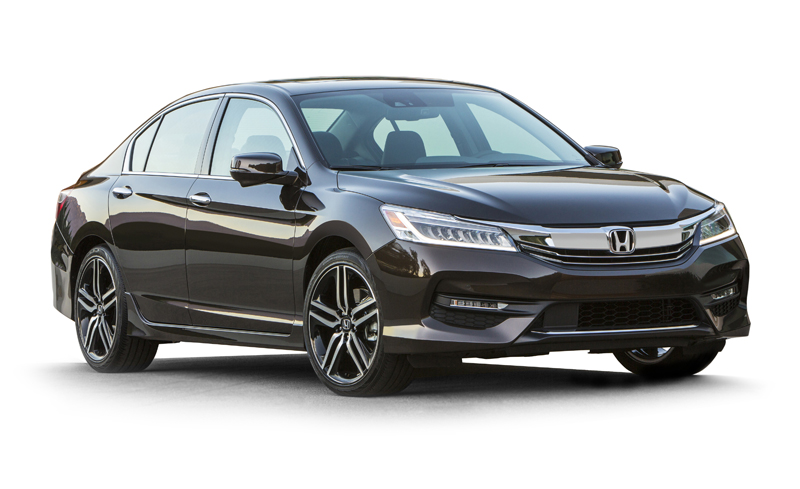
\includegraphics[width=2.7in]{accord.jpg}
\end{figure}

The 2016 Honda Accord sells at many different dealerships in New York City but sell it for more and some for less. We'll assume that the final negotiated price is distributed normally because it's most likely the sum of many different negotiation factors.

Our goal here is to determine the mean price at a certain car dealership in Astoria that people have been saying is \qu{too cheap} and if it's too cheap, Honda corporate may wish to investigate.


\begin{enumerate}



\easysubproblem{Assume that each Accord's price at the Astoria dealership is normal and $\iid$ given the parameters. Is this a good model? Why or why not? There is no \qu{correct} answer here but I expect you to defend whatever answer you write using the concepts we discussed in class.} \spc{6}

\easysubproblem{Despite what you wrote in (b), assume $\iid$ for the rest of the problem. The nationwide variance for a Honda Accord selling price we're going to assume is $\sigsq = \$1000^2$. Given a sample with average $\xbar$ and sample size $n$, what is the distribution of the mean price of a car from this shady Astoria dealership? Assume an uninformative prior of your choice but ensure to explicitly state it.}\spc{5}

\easysubproblem{You and your colleague go down to the Astoria dealership undercover and ask to buy a Honda. After much negotiation, they will sell it to you for \$19,000 and they will sell it to your colleague for \$18,200 but they sense something suspicious so you hesitate to send another one of your guys down there to do another faux negotiation. Unfortunately, we're going to have to estimate the mean with just $x_1=19000$ and $x_2 = 18200$. What is your best guess of the mean price of Honda Accords sold here? Assume your prior from (a). \compexpl }\spc{2}

\easysubproblem{What is the shrinkage value (which we have been denoting $\rho$) for this estimate? \compexpl}\spc{3}

\intermediatesubproblem{Based on this data, we wish to test if this dealership is selling Honda Accords below the manufacturer sugested retail price (MSRP) of \$22,205 --- if so, they would be subject to a fine. Calculate a $p$-value for this test below by using notation from Table~\ref{tab:eqs} but do not solve numerically.}\spc{4}

\intermediatesubproblem{What is the probability I get a really good deal --- that I can buy a car from these Astoria people for under \$17,000? Use the notation from Table~\ref{tab:eqs} but do not solve numerically.}\spc{3}



\end{enumerate}

\problem This question is about building a model to understand the accuracy of this beverage-filling machine pictured below:

\begin{figure}[htp]
\centering
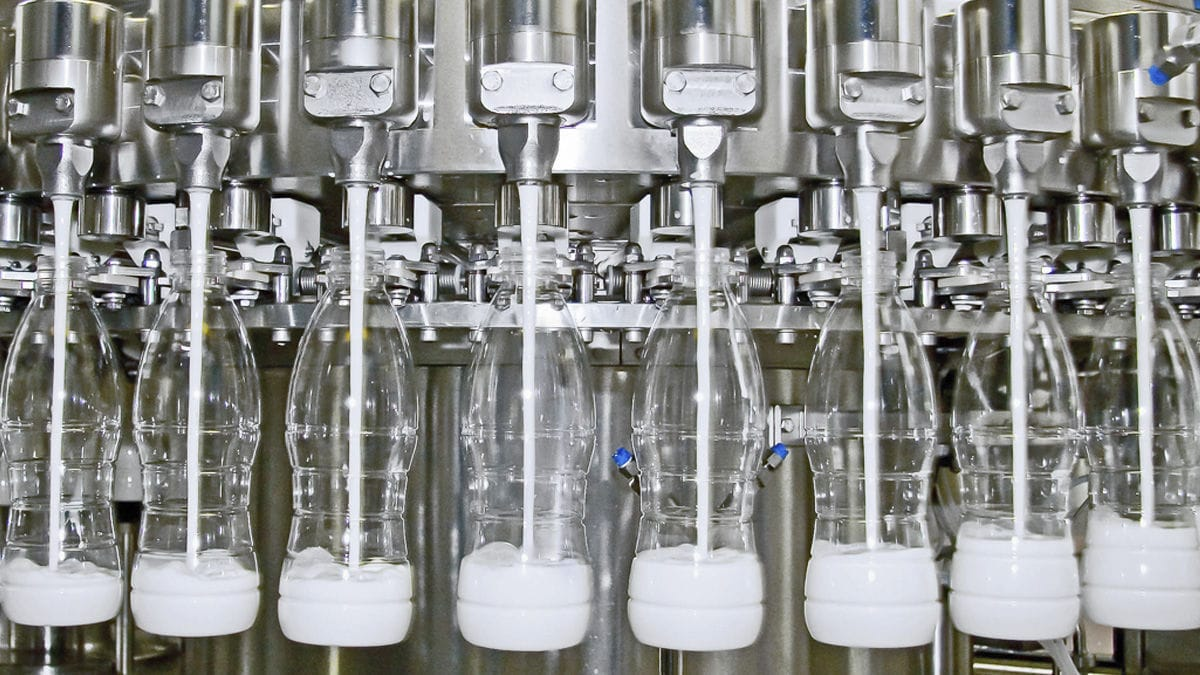
\includegraphics[width=3.7in]{milk_filling.jpg}
\end{figure}

This machine fills 12oz plastic bottles. There is no doubt the mean amount of liquid filled per bottle is 12oz as been determined by the final weights of pallets of filled bottles. But we are uncertain about the variance. We decide to do an experiment and select $n = 21$ bottles at random and measure the amount of liquid in each bottle. Here are the measurements:

\begin{verbatim}
                   12.00 12.05 11.98 11.66 12.05 11.92 12.03
                   12.23 12.36 11.57 12.04 12.10 11.99 12.47
                   12.57 11.83 12.20 12.48 12.14 12.14 12.74
\end{verbatim}

\begin{enumerate}

\easysubproblem{Write a model below for the amount of milk in each of the $n$ bottles. Hint: use the normal model!}\spc{3}

\easysubproblem{Find the MLE for $\sigsq$.}\spc{3}

\easysubproblem{Under the Jeffrey's prior for $\sigsq$, find the posterior of $\sigsq$ by solving for the parameter values.}\spc{3}

\intermediatesubproblem{Find a left-sided credible region for $\sigsq$. This will give the upper bound for the machine's variance.}\spc{3}


\intermediatesubproblem{The bottles are actually 13.5oz. This means that you wish to test if $\sigsq > 0.352$ for if so, about 1/100,000 of the bottles will be overfull and that's the tolerance of the factory. Do this test.}\spc{6}


\intermediatesubproblem{Find the probability the next bottle has more than 13oz of liquid.}\spc{3}

\end{enumerate}



\end{document}





